\documentclass[legalpaper]{article}

\usepackage[utf8]{inputenc}
\usepackage[T1]{fontenc}
\usepackage[spanish]{babel}
\usepackage{graphicx}
\usepackage{caption}
\usepackage{geometry}
\geometry{margin=2cm}

\title{Práctica 3 -- Sistemas de Control II}
\author{Emerson Warhman}
\date{}

\begin{document}

% \maketitle

\section*{\centering Resultados}
\setcounter{figure}{1}

\begin{figure}[h!]
    \centering
    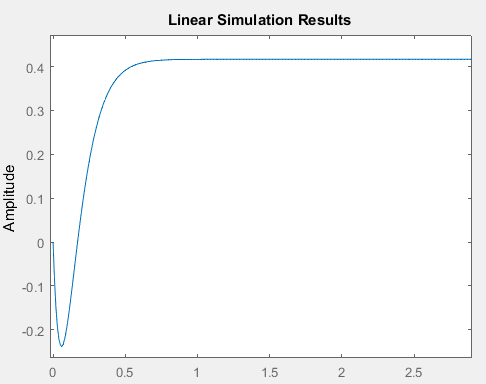
\includegraphics[width=0.9\linewidth]{imagenes/2-respuesta-a-la-entrada-escalon.png}
    \caption{Respuesta a la entrada escalón}
    \label{fig:2-respuesta-a-la-entrada-escalon}
\end{figure}

\begin{figure}[h!]
    \centering
    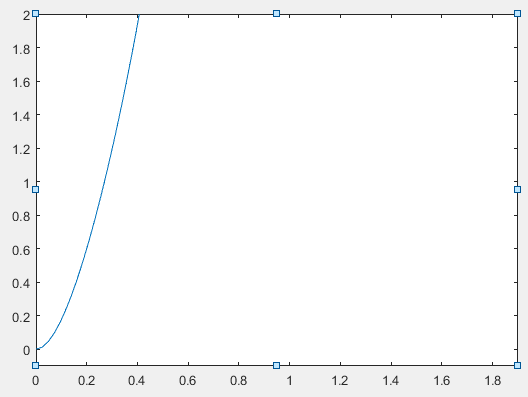
\includegraphics[width=0.9\linewidth]{imagenes/3-X1_vs_X2.png}
    \caption{Gráfico de X1 vs X2}
    \label{fig:3-X1_vs_X2}
\end{figure}

\begin{figure}[h!]
    \centering
    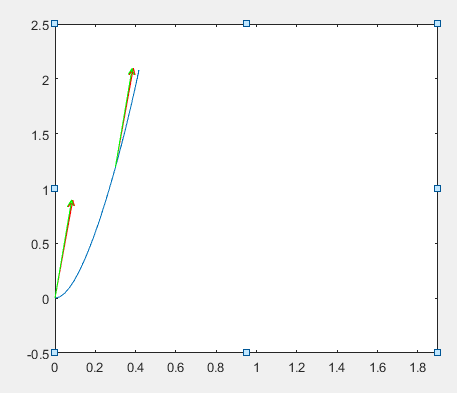
\includegraphics[width=0.9\linewidth]{imagenes/5-Comparacion-estados-X1-X2-con-autovectores.png}
    \caption{Comparación estados X1 X2 con autovectores}
    \label{fig:5-Comparacion-estados-X1-X2-con-autovectores}
\end{figure}

\begin{figure}[h!]
    \centering
    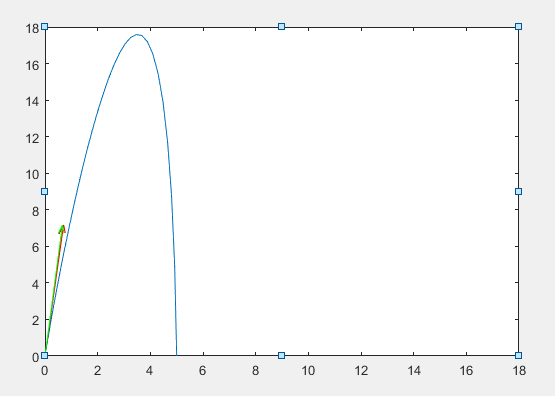
\includegraphics[width=0.9\linewidth]{imagenes/6-trayectoria-X2-vs-X1-respuesta-natural.png}
    \caption{Trayectoria X2 vs X1 respuesta natural con condiciones iniciales (4, 0)}
    \label{fig:6-trayectoria-X2-vs-X1-respuesta-natural}
\end{figure}

\begin{figure}[h!]
    \centering
    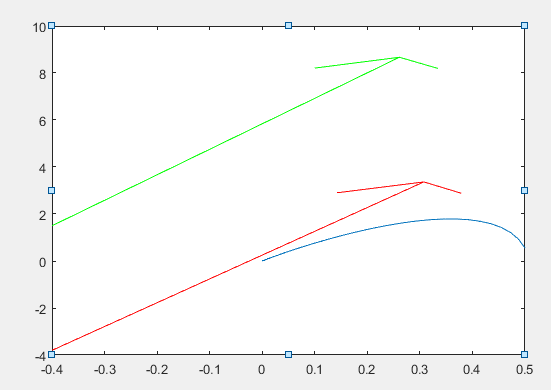
\includegraphics[width=0.9\linewidth]{imagenes/7-2-trayectoria-x1-x2-condiciones-iniciales-0.5-0.55.png}
    \caption{Trayectoria x1 x2 condiciones iniciales (0.5, 0.55)}
    \label{fig:7-2-trayectoria-x1-x2-condiciones-iniciales-0-5-0-55}
\end{figure}

\begin{figure}[h!]
    \centering
    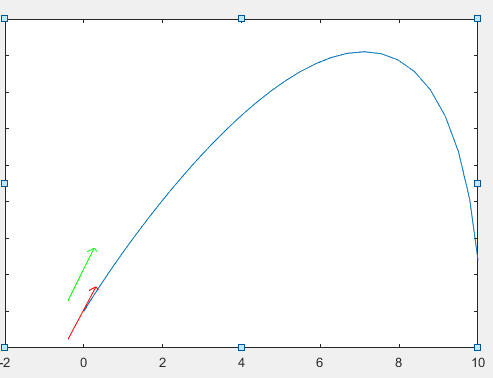
\includegraphics[width=0.9\linewidth]{imagenes/7-3-trayectoria-x1-x2-condiciones-iniciales-10-7.png}
    \caption{Trayectoria x1 x2 condiciones iniciales (10, 7)}
    \label{fig:7-3-trayectoria-x1-x2-condiciones-iniciales-10-7}
\end{figure}

\begin{figure}[h!]
    \centering
    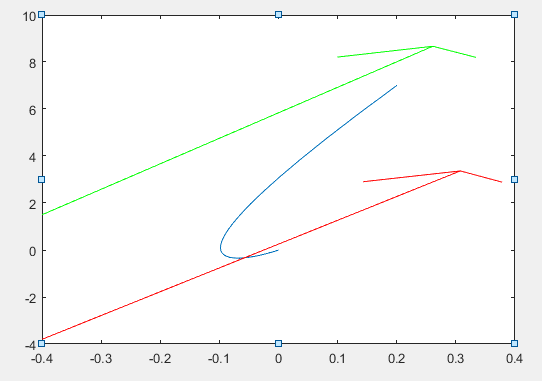
\includegraphics[width=0.9\linewidth]{imagenes/7-4-trayectoria-X1-X2-condiciones-iniciales-0.2-7.png}
    \caption{Trayectoria X1 X2 condiciones iniciales (0.2, 7)}
    \label{fig:7-4-trayectoria-X1-X2-condiciones-iniciales-0-2-7}
\end{figure}

\begin{figure}[h!]
    \centering
    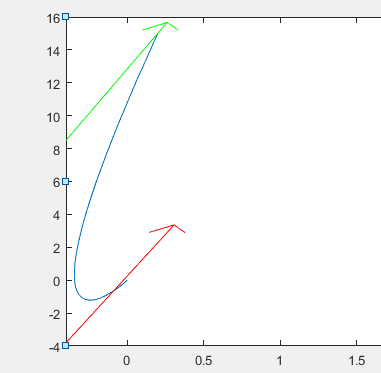
\includegraphics[width=0.9\linewidth]{imagenes/7.5-trayectoria-X1-X2-condiciones-iniciales-0,2-15.png}
    \caption{Trayectoria X1 X2 condiciones iniciales (0.2, 15)}
    \label{fig:7-5-trayectoria-X1-X2-condiciones-iniciales-0-2-15}
\end{figure}

\begin{figure}[h!]
    \centering
    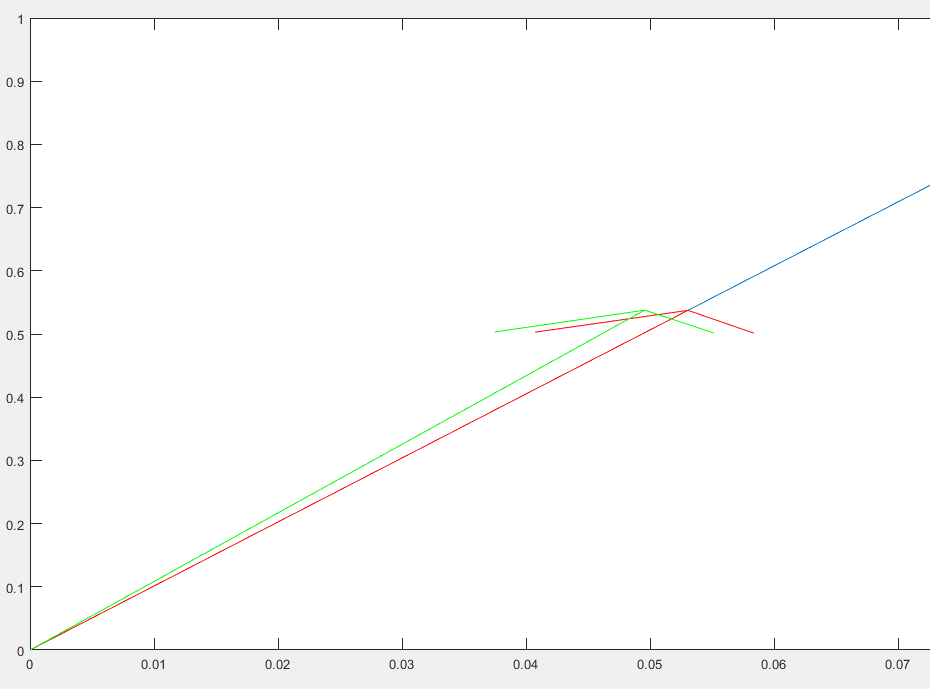
\includegraphics[width=0.9\linewidth]{imagenes/8.1-condiciones-iniciales-autovector-1.png}
    \caption{Trayectoria X1 X2 al aplicar condiciones iniciales del autovector 1}
    \label{fig:8-1-condiciones-iniciales-autovector-1}
\end{figure}

\begin{figure}[h!]
    \centering
    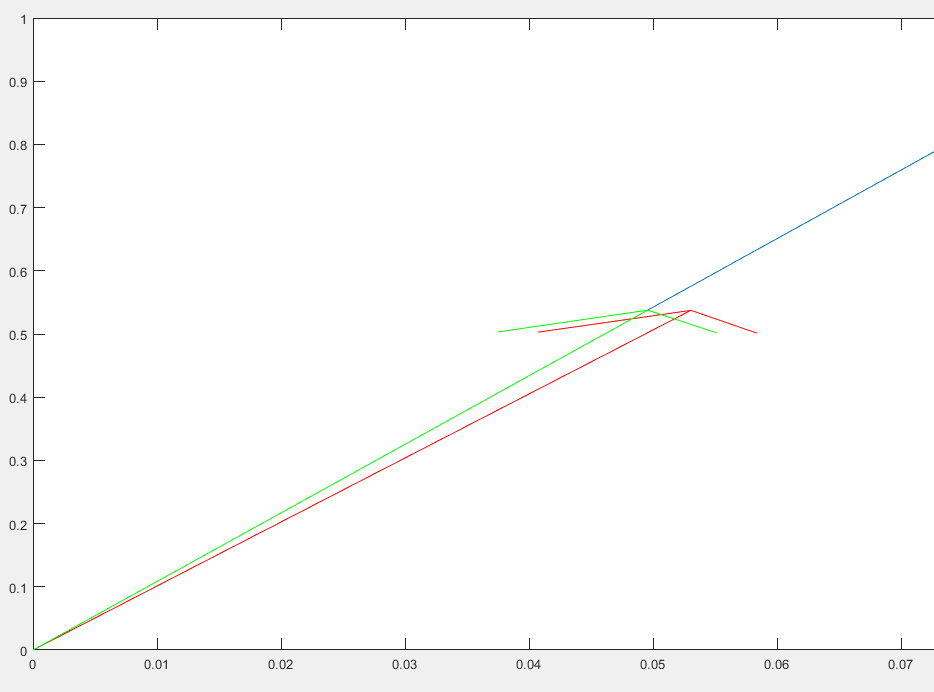
\includegraphics[width=0.9\linewidth]{imagenes/8.2-condiciones-iniciales-autovector-2.png}
    \caption{Trayectoria X1 X2 al aplicar condiciones iniciales del autovector 2}
    \label{fig:8-2-condiciones-iniciales-autovector-2}
\end{figure}

\begin{figure}[h!]
    \centering
    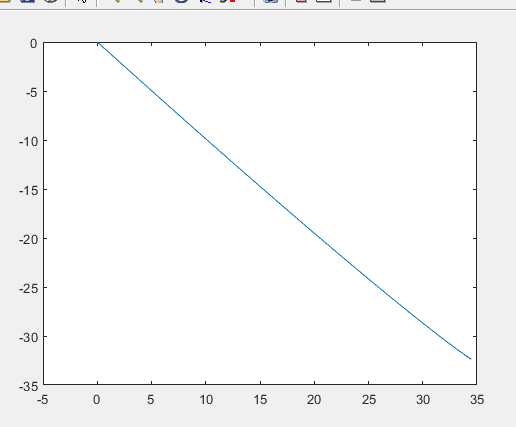
\includegraphics[width=0.9\linewidth]{imagenes/9-trayectoria-d1-d2-de-la-representacion-canonica.png}
    \caption{Trayectoria d1 vs d2 de la representación canónica}
    \label{fig:9-trayectoria-d1-d2-de-la-representacion-canonica}
\end{figure}

\begin{figure}[h!]
    \centering
    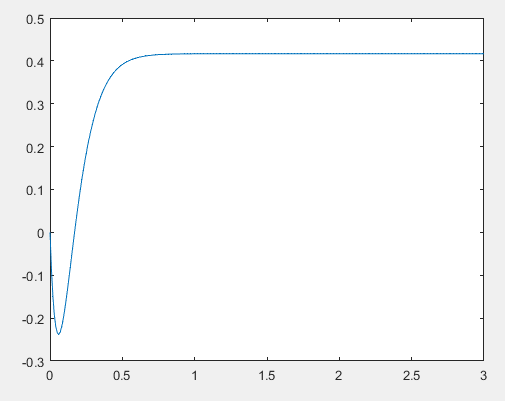
\includegraphics[width=0.9\linewidth]{imagenes/10-2-respuesta del sistema-reconstruida.png}
    \caption{Respuesta del sistema usando la salida reconstruida W*D}
    \label{fig:10-2-respuesta-del-sistema-reconstruida}
\end{figure}

\begin{figure}[h!]
    \centering
    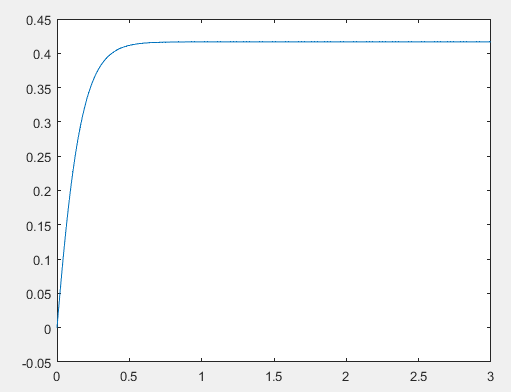
\includegraphics[width=0.9\linewidth]{imagenes/10-1-t-vs-x1-del-sistema-W-por-D.png}
    \caption{comportamiento del estado X1 vs tiempo del sistema W por D}
    \label{fig:10-1-t-vs-x1-del-sistema-W-por-D}
\end{figure}

\begin{figure}[h!]
    \centering
    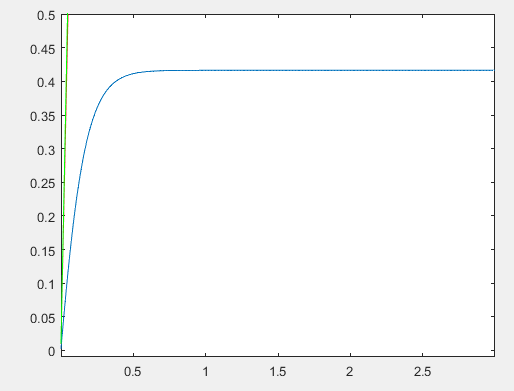
\includegraphics[width=0.9\linewidth]{imagenes/10-3-t-vs-x1-del-sistema-originalmente.png}
    \caption{Comportamiento del estado X1 vs tiempo del sistema originalmente}
    \label{fig:10-3-t-vs-x1-del-sistema-originalmente}
\end{figure}

\end{document}

